\documentclass[aspectratio=169]{beamer}
\usepackage[utf8]{luainputenc}
\usepackage{amssymb,amsmath}
\usepackage{graphicx}
\usepackage{tikz}
\usepackage{beamercolorthemetud}
\usepackage[backend=biber]{biblatex}
\usepackage{caption}
\captionsetup[figure]{font=scriptsize}
\usepackage{hyperref}

\usepackage{subcaption}
\usepackage[absolute,overlay]{textpos}
  \setlength{\TPHorizModule}{1mm}
  \setlength{\TPVertModule}{1mm}




\addbibresource{bibl.bib}
\setbeamertemplate{bibliography item}{\insertbiblabel}
\usepackage[english]{babel}
\usetheme[]{tud}
\setbeamercolor{background canvas}{bg=}
\setbeamerfont{frametitle}{size=\Large}
\input{macros}



\title{MeetForSport: Adaptation Concept}
\author{Mattis Lahr, Felix Fischer}
\date{10.12.2021}

\einrichtung{\hspace{-1pt}Institute of Systems Architecture}
\datecity{Dresden}




\AtBeginSection[]{\partpage{\usebeamertemplate***{part page}}}
\begin{document}
\maketitle



\begin{frame}
    \frametitle{Table of Contents}
    \tableofcontents
\end{frame}




\section{Problematic Situations}
\begin{frame}   
	\frametitle{Situation 1:  Bad or no internet connection}
	 \begin{figure}
		\centering
		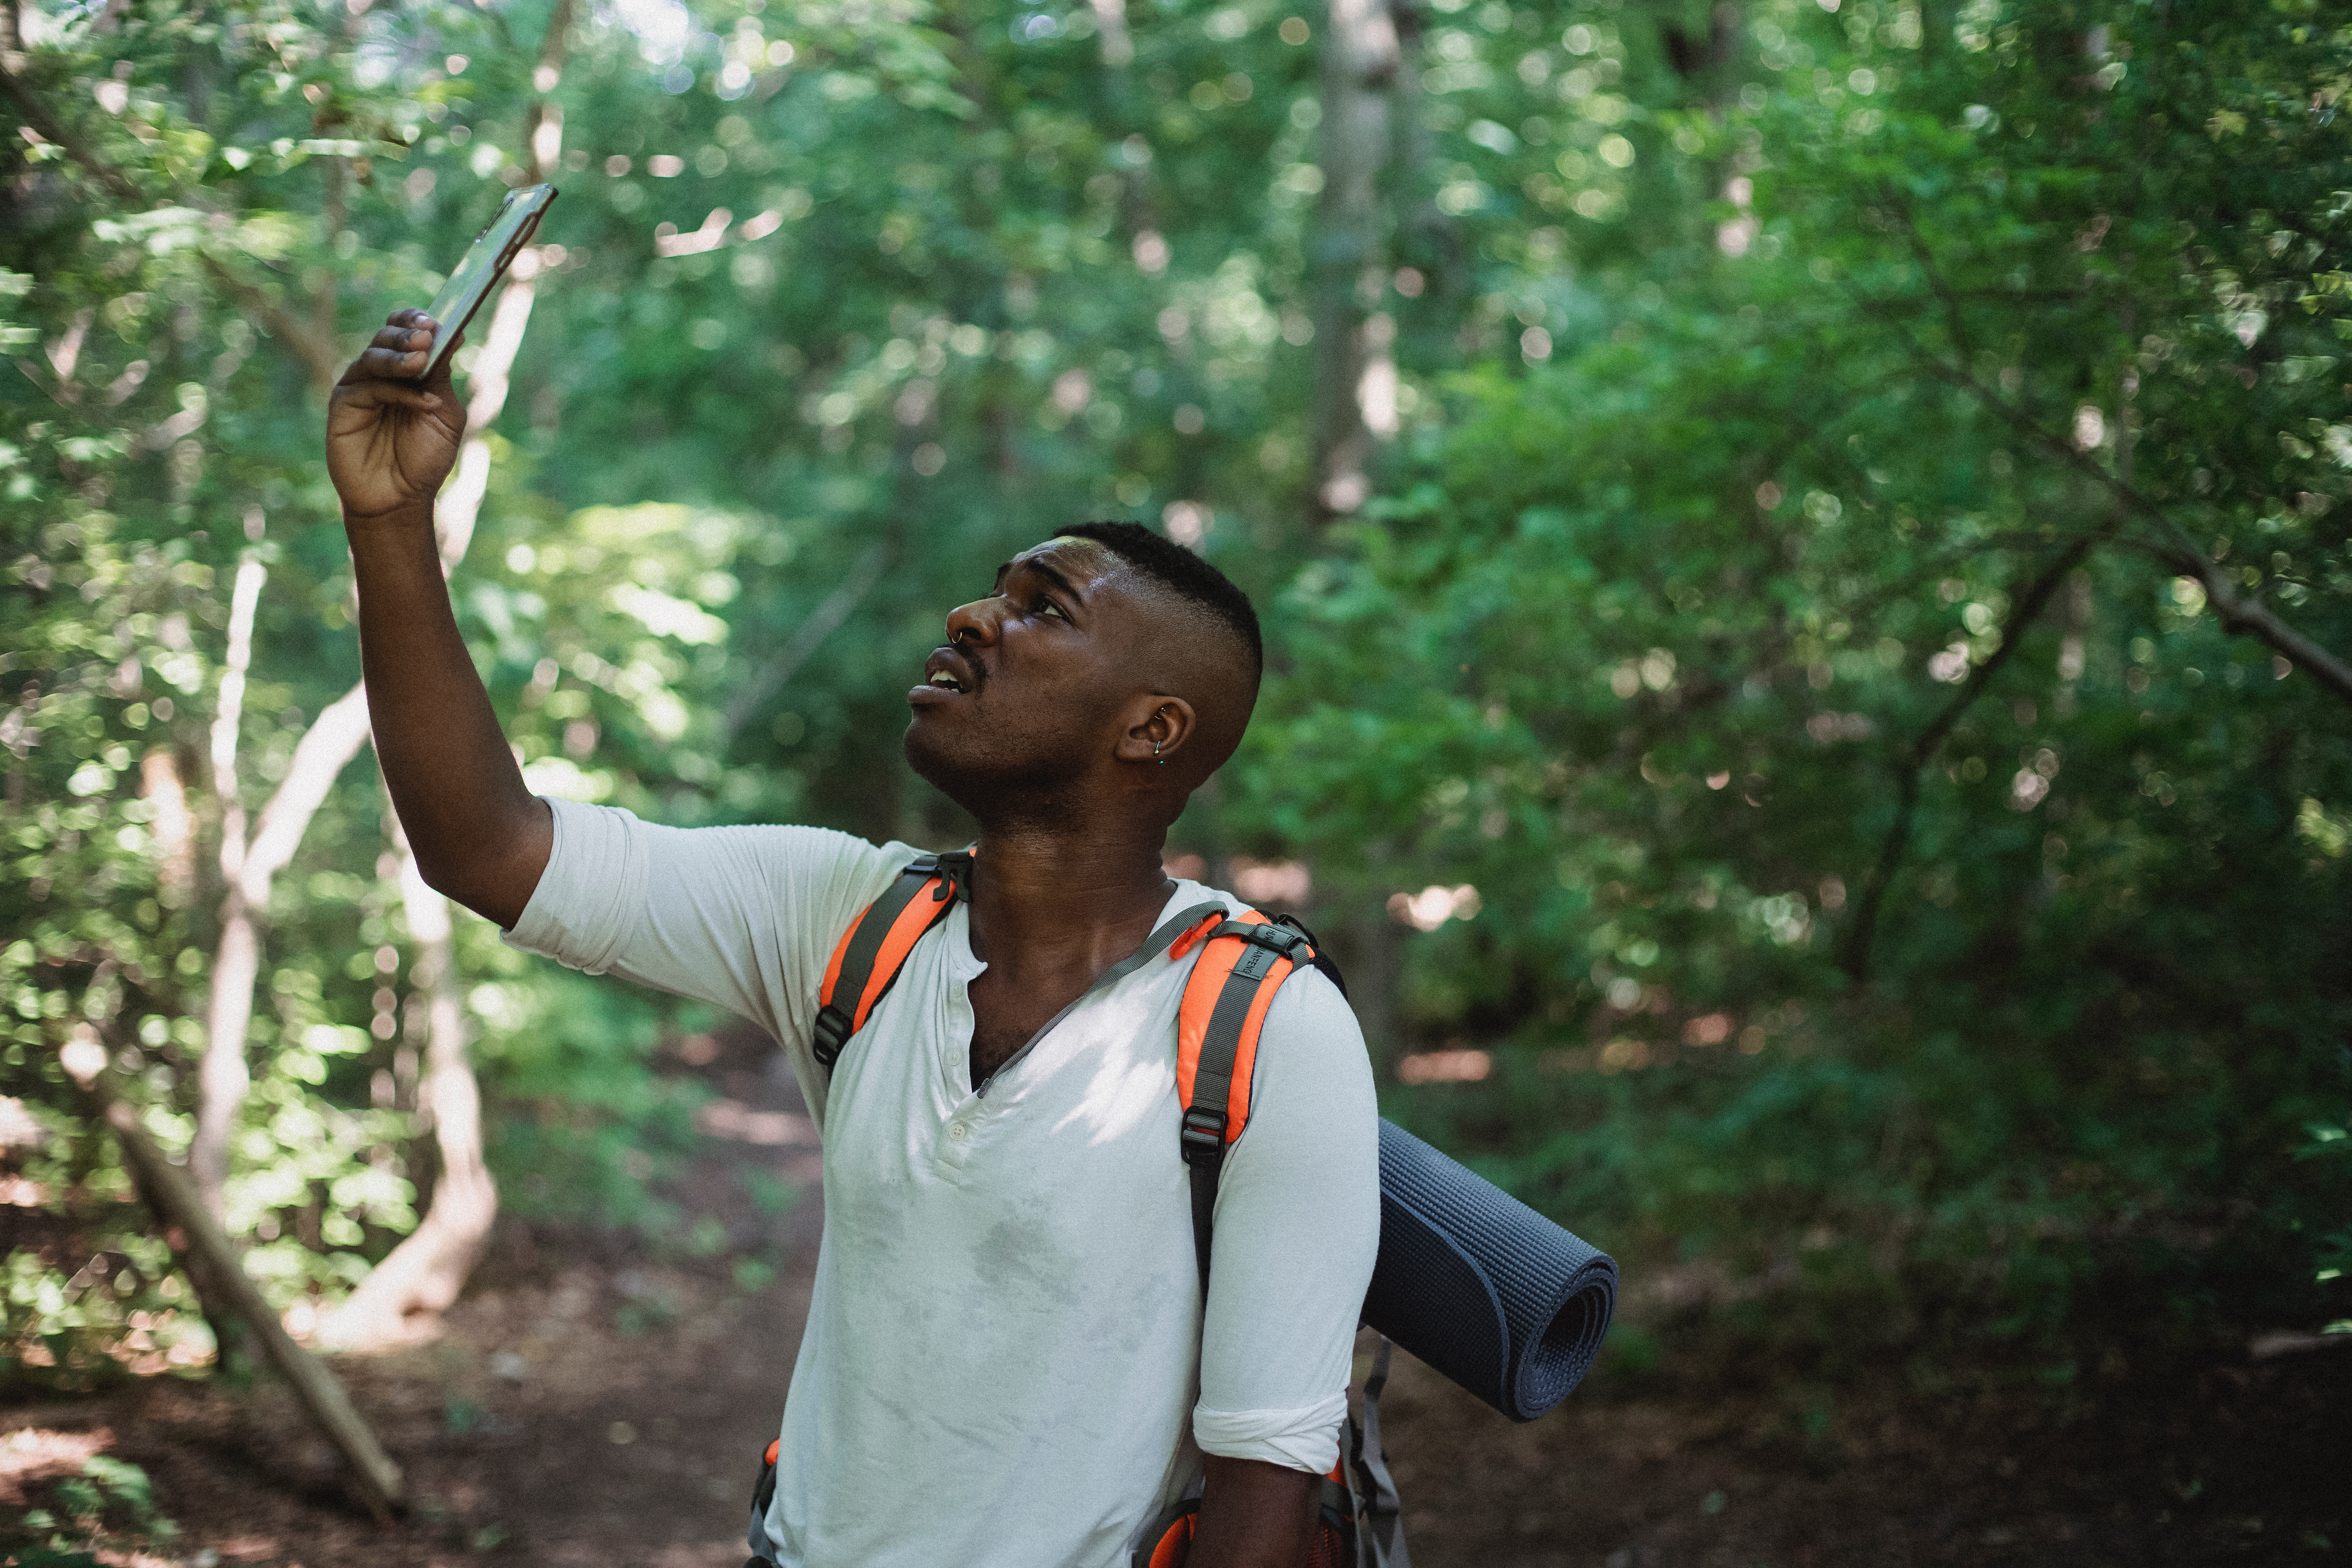
\includegraphics[width=0.6\textwidth]{media/no_internet.jpg}
	\end{figure}
\end{frame}
\begin{frame}   
	\frametitle{Situation 2: low battery}
	 \begin{figure}
		\centering
		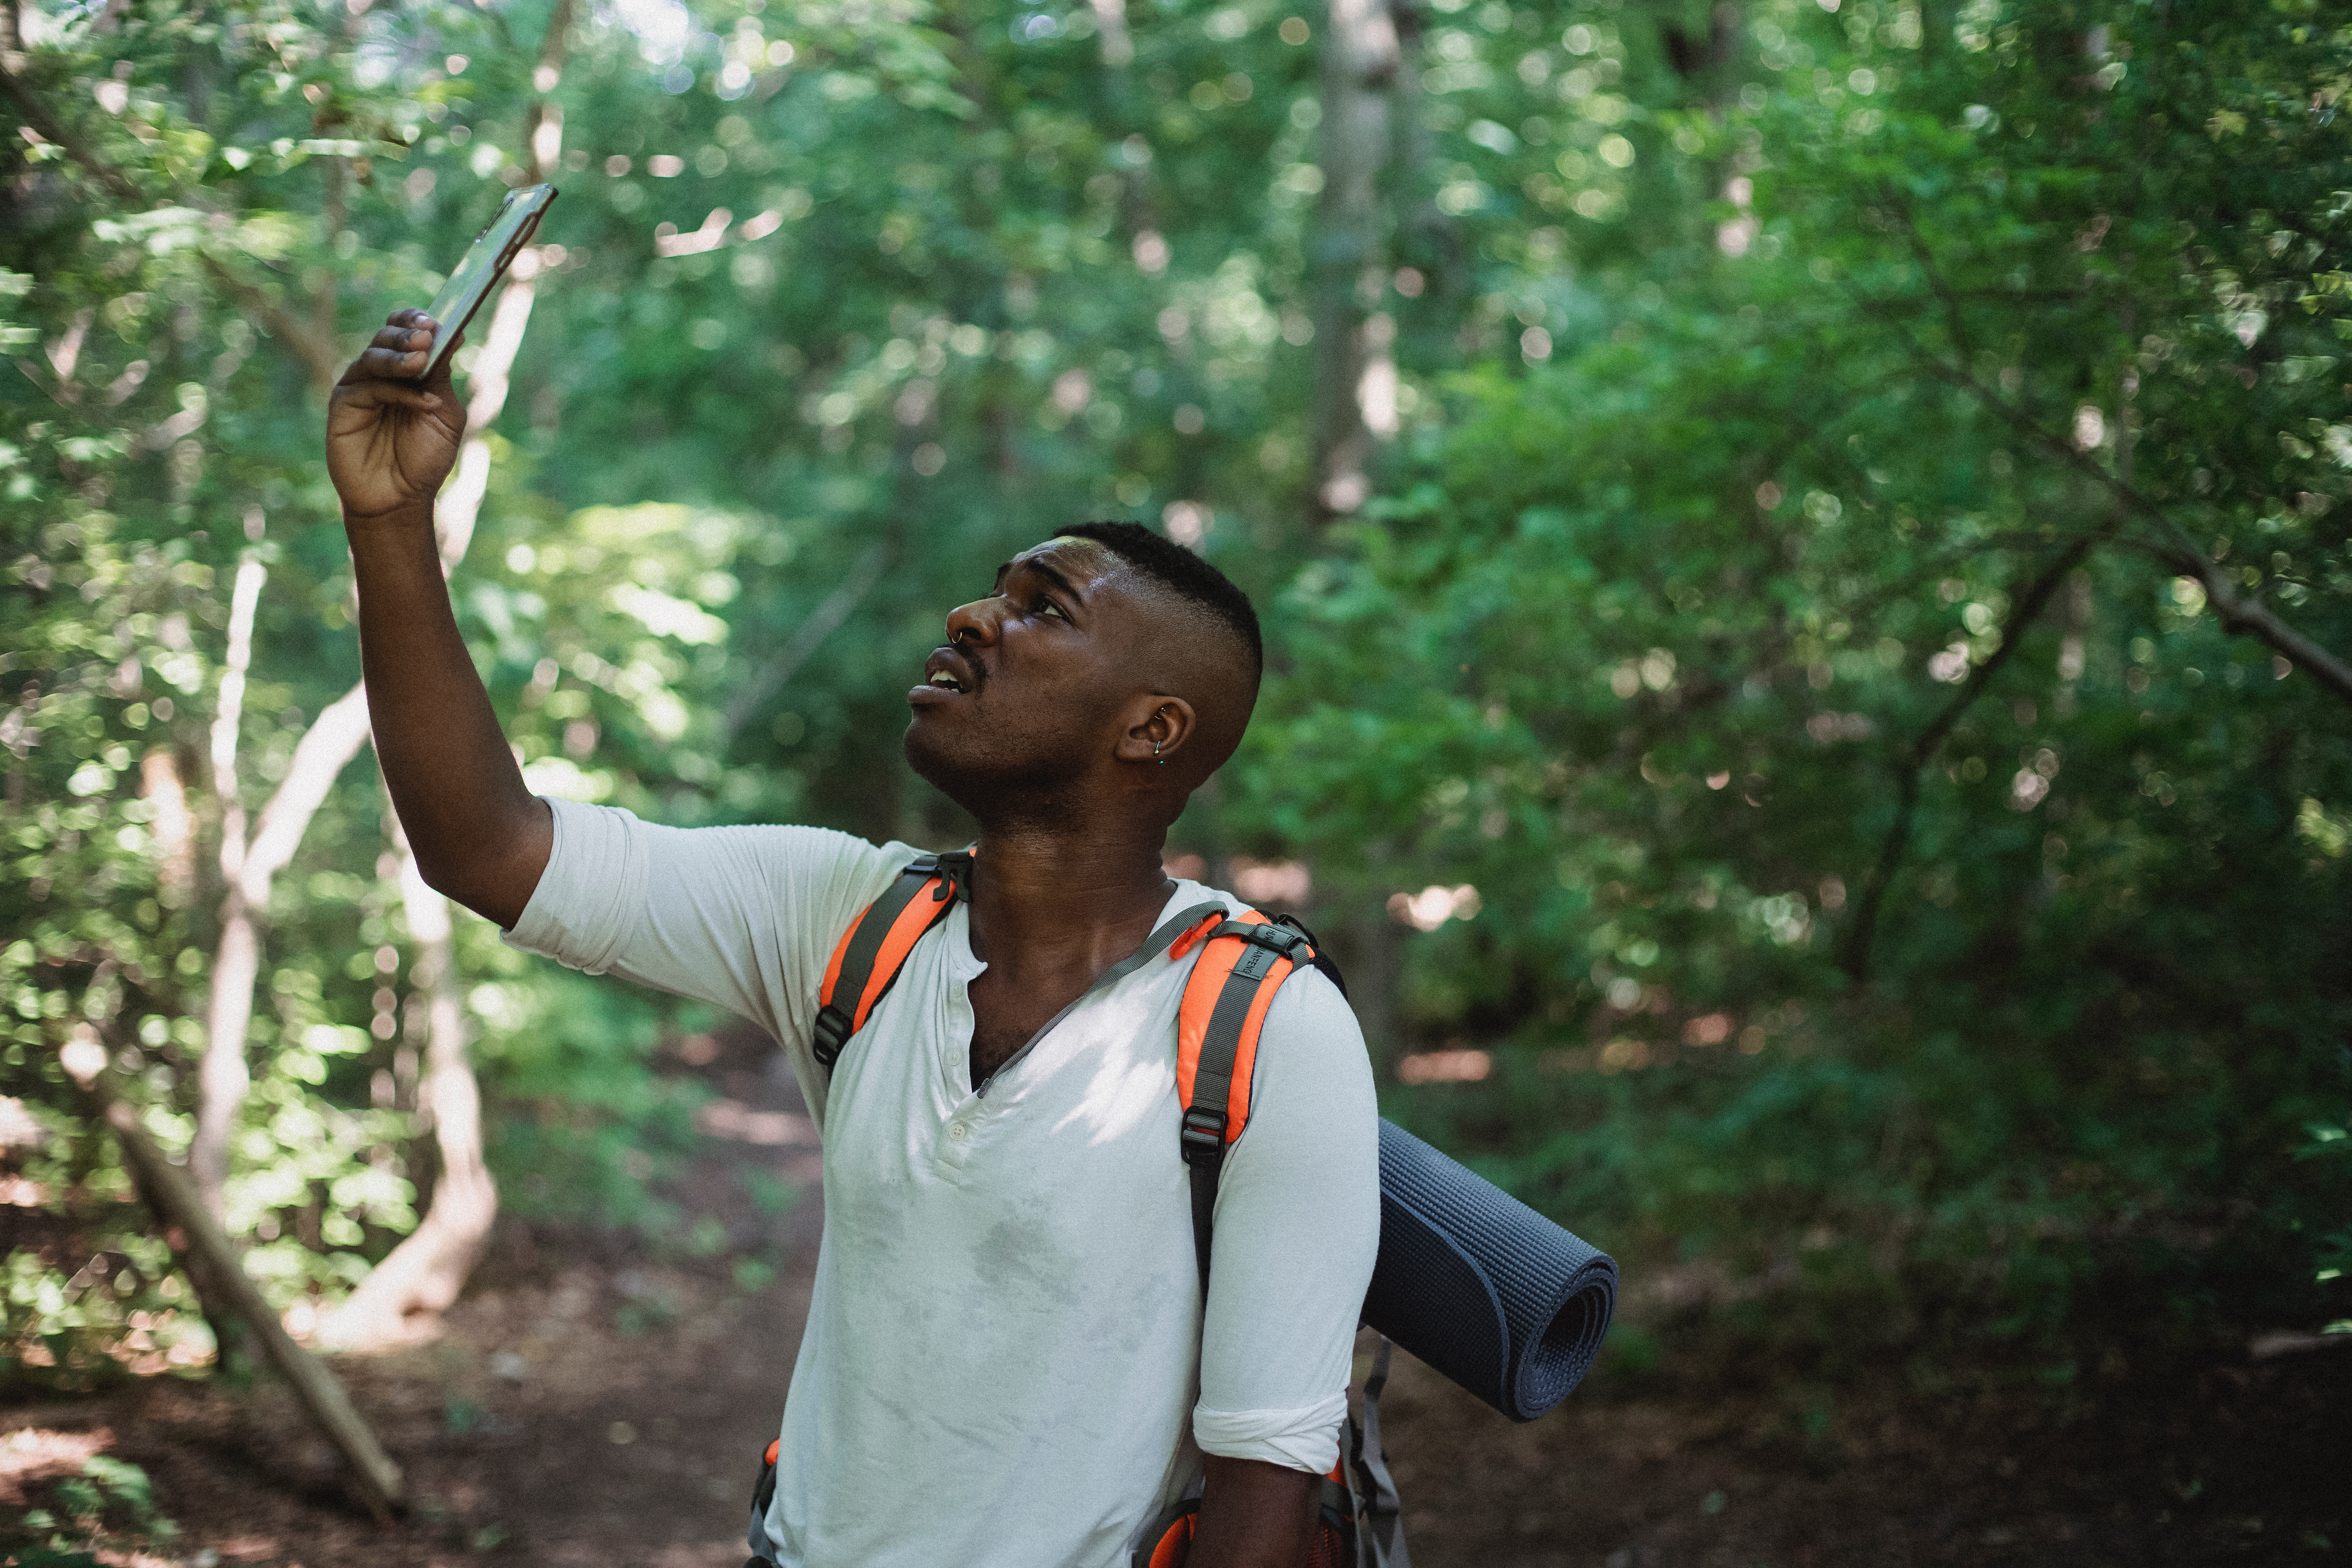
\includegraphics[width=0.6\textwidth]{media/no_internet.jpg}
	\end{figure}
\end{frame}




\section{Context Features}
\begin{frame}   
	\frametitle{Context features to control our adaptation}
\end{frame}




\section{Adaptation Mechanisms}
\begin{frame}   
	\frametitle{Adaptation Mechanisms}
\end{frame}




\section{MAPE-K}
\begin{frame}   
	\frametitle{MAPE-K}
\end{frame}




\section{Detailed Architecture and Technology Choice}
\begin{frame}
	\frametitle{Detailed architecture and technology choice}
\end{frame}



\end{document}